% !TeX program = lualatex
\RequirePackage{iftex}
\ifLuaTeX
  \documentclass[a4paper,11pt]{ltjsarticle}
  \usepackage{luatexja-fontspec}
  \defaultjfontfeatures{Scale=0.924715,Kerning=Off,Script=CJK,CJKShape=JIS2004,
    YokoFeatures={JFM=ujis},TateFeatures={JFM=ujisv}}
  \setmainjfont[BoldFont=HaranoAjiMincho-Bold.otf]{HaranoAjiMincho-Regular.otf}
  \setsansjfont[BoldFont=HaranoAjiGothic-Bold.otf]{HaranoAjiGothic-Regular.otf}
\else
  \documentclass[a4paper,11pt,xelatex,ja=standard,jafont=haranoaji]{bxjsarticle}
\fi
\usepackage{geometry}
\geometry{margin=25mm}
\usepackage{lmodern}
\usepackage{amsmath,amssymb,amsthm,bm}
\usepackage{booktabs,tabularx,array,graphicx,tikz}
\usetikzlibrary{arrows.meta,positioning,calc}
\usepackage{algorithm,algpseudocode}
\usepackage[round,authoryear]{natbib}
\usepackage{xurl}
\usepackage[unicode,hidelinks]{hyperref}
\usepackage{bookmark}
\hypersetup{pdftitle={解釈可能な深層ベクトル自己回帰によるGranger非因果推定},pdfauthor={栗田 煌矢}}
\newtheorem{proposition}{命題}[section]
\theoremstyle{definition}
\newtheorem{definition}[proposition]{定義}
\renewcommand{\proofname}{証明}
\floatname{algorithm}{Algorithm}
\algrenewcommand\algorithmicrequire{\textbf{入力:}}
\algrenewcommand\algorithmicensure{\textbf{出力:}}
\newcommand{\E}{\mathbb{E}}
\newcommand{\R}{\mathbb{R}}
\newcommand{\ind}{\mathbf{1}}
\newcommand{\norm}[1]{\left\lVert #1\right\rVert}
\DeclareMathOperator{\median}{median}
\DeclareMathOperator{\sign}{sign}
\setcounter{tocdepth}{2}
\setlength{\emergencystretch}{2em}
\linespread{1.08}
\raggedbottom
\title{\LARGE 解釈可能な深層ベクトル自己回帰による\\グレンジャー非因果推定}
\author{栗田 煌矢\\東北大学経済学部 李研究室}
\date{}
\begin{document}
\pagenumbering{roman}
\maketitle
% !TeX root = ../main.tex
\begin{abstract}
非線形な多変量時系列の依存構造と関係の方向を記述するため、入力依存係数と構造ゲートを持つGSE-VARを提案する。係数生成の入力と出力を共通ゲートで選択し、全ラグのゲートが\(0\)なら推定モデルの予測がその系列に依存しないことを示す。各経路をBernoulliゲートで表し、選択確率の和に罰則を課す期待L0正則化と、DisARMによる不偏勾配推定を用いて学習する。独立な予備系列で設定を選んだLorenz96では、系列長250の平均F1が\(0.997\)となり、系列長500では全5系列で参照構造を回復した。線形VARの系列長500では平均符号BA\(0.975\)を得た。付録ではFavoritaの12商品カテゴリに適用する。検証MSEで選んだモデルは7本の非自己辺を選択し、標準化尺度のテストMSEは\(0.4620\)であった。選択した経路を、観測条件下の予測依存として記述する。
\end{abstract}

\clearpage
\pagenumbering{arabic}
\section{序論}
\label{sec:introduction}
経済活動や需要の多変量時系列では、他の情報を条件とした予測上の必要性から系列間の関係を調べるグレンジャー因果分析が用いられる\citep{granger1969}。線形ベクトル自己回帰（VAR）は係数から関係を読めるが、非線形モデルでは入力が予測に関与する複数の経路を制御する必要がある。

この課題に対し、\citet{tank2022}は入力層の構造正則化によって依存構造を抽出した。一方、一般化VAR（generalised VAR; GVAR）は、過去値を入力依存の係数で重み付けし、非線形な関係を係数として表す\citep{marcinkevics2021}。この係数表現で不要な入力を除くには、過去値に掛かる係数だけでなく、その入力が他の係数を変える経路も制御する必要がある。

そこでGated Self-Explaining VAR（GSE-VAR）を提案する。対象・入力・ラグ別の共通ゲートで係数生成の入力と出力を制御し、各ゲートの選択確率に期待L0正則化を課し、DisARMで期待損失のロジット勾配を推定する。係数生成器とロジットはAdamで同時に更新する。

本研究の貢献は、非線形な係数表現と、ゲートの\(0\)による入力非依存性の判定を両立する設計にある。十分条件と符号解釈を示し、Lorenz96の構造回復と線形VARの符号回復から評価する。さらに付録\ref{sec:application}では、Favoritaの販売系列を用いて、正解構造が未知の場合のモデル選択とカテゴリ間関係の記述を例示する。

\section{関連研究}
\label{sec:related}
Neural Granger Causality（NGC）は対象別ネットワークの入力重みを正則化して入力経路を除去する\citep{tank2022}。GVARは入力依存係数によって非線形な関係を表す\citep{marcinkevics2021}。提案手法は、係数値と係数生成入力を共通ゲートで制御し、入力除去と係数表現を結び付ける。提案手法ではBernoulliゲートによって経路を選択し、対の標本を用いるDisARM\citep{dong2020}でロジット勾配を推定する。共通ゲートの設計により、二値選択と入力依存係数の表現を結び付ける。

\section{問題設定}
\label{sec:problem}


\subsection{予測依存構造}
\(p\)変量時系列を\(\bm x_t=(x_{1,t},\ldots,x_{p,t})^\top\)、最大ラグを\(K\)、利用する過去を\(\bm X_t=(\bm x_{t-1},\ldots,\bm x_{t-K})\)とする。本研究は二乗誤差による予測を扱うため、対象を条件付き平均
\(\mu_i(\bm X_t)=\E[x_{i,t}\mid\bm X_t]\)とし、その近似を\(\widehat x_{i,t}=h_i(\bm X_t)\)と書く。

\begin{definition}[条件付き平均に関する非因果性]
\(\bm X_t^{(-j)}\)を、\(\bm X_t\)から系列\(j\)の全ラグを除いた情報とする。
\begin{equation}
 \E[x_{i,t}\mid\bm X_t]
 =
 \E[x_{i,t}\mid\bm X_t^{(-j)}]
 \quad\text{a.s.}
 \label{eq:mean-noncausality}
\end{equation}
が成立するとき、系列\(j\)の過去は系列\(i\)の条件付き平均の予測を改善しない。
\end{definition}

式\eqref{eq:mean-noncausality}が対象とするのは条件付き平均の依存性である。これに対応するモデル上の性質として、他の入力を固定して系列\(j\)の過去を変えても\(h_i\)が変わらないことを非因果性と定める。

\subsection{線形VARと係数表現}
線形VARの予測式は
\begin{equation}
 \widehat{\bm x}_t=\bm b+\sum_{k=1}^{K}A_k\bm x_{t-k}
 \label{eq:linear-var}
\end{equation}
である。この形式では、全\(k\)について\((A_k)_{ij}=0\)なら系列\(j\)の過去を含む項が全て消え、予測はその系列に依存しない。隣接行列は行を予測対象、列を入力とし、\(\widehat A_{ij}=1\)を\(j\to i\)の向きと定める。

入力依存係数では係数生成を通じた依存も遮断する必要がある。

\section{提案モデル}
\label{sec:model}
\subsection{係数生成入力と出力の共通ゲート}
予測対象\(i\)、ラグ\(k\)に対し、入力系列ごとのゲート
\(\bm g_{ki}=(g_{ki1},\ldots,g_{kip})^\top\)と、独立した係数生成器
\(f_{\theta_{ki}}:\R^p\to\R^p\)を設ける。GSE-VARを
\begin{align}
 \bm v_{ki,t}&=\bm g_{ki}\odot\bm x_{t-k},\notag\\
 \bm c_{ki,t}&=\bm g_{ki}\odot f_{\theta_{ki}}(\bm v_{ki,t}),\label{eq:gated-coefficients}\\
 \widehat x_{i,t}&=b_i+\sum_{k=1}^{K}\bm c_{ki,t}^{\top}\bm x_{t-k}
 \label{eq:gse-var}
\end{align}
で定義する。\(\odot\)は要素積、\(b_i\)は入力に依存しない切片、\(\bm c_{ki,t}\)はゲートを含めた有効係数である。ゲートは時点によらない二値変数\(g_{kij}\in\{0,1\}\)とする。

係数生成器は対象・ラグ別の多層パーセプトロン（MLP）とする。同一ラグ内の選択入力間の交互作用を表し、ラグ間は加算で集約する。

\begin{figure}[H]
\centering
\begin{tikzpicture}[>=Stealth,font=\small,
 box/.style={draw,rounded corners=1pt,minimum height=10mm,align=center},
 every node/.style={inner sep=4pt}]
 \node[box,minimum width=16mm] (x) at (0,0) {\(\bm x_{t-k}\)};
 \node[box,minimum width=19mm] (in) at (2.3,0) {入力の選択\\\(\bm v_{ki,t}\)};
 \node[box,minimum width=20mm] (f) at (4.9,0) {係数生成\\\(f_{\theta_{ki}}\)};
 \node[box,minimum width=19mm] (out) at (7.6,0) {出力の選択\\\(\odot\,\bm g_{ki}\)};
 \node[box,minimum width=16mm] (c) at (10,0) {\(\bm c_{ki,t}\)};
 \node[box,fill=gray!8,minimum width=24mm] (g) at (4.9,1.7) {共通の構造ゲート\\\(\bm g_{ki}\)};
 \node[box,minimum width=29mm] (y) at (10,-1.9) {内積・ラグ方向の和\\\(\widehat x_{i,t}\)};
 \draw[->] (x)--(in);
 \draw[->] (in)--(f);
 \draw[->] (f)--(out);
 \draw[->] (out)--(c);
 \draw[->] (g.west)-|(in.north);
 \draw[->] (g.east)-|(out.north);
 \draw[->] (c)--(y);
 \draw[->] (x.south)|-(y.west);
\end{tikzpicture}
\caption{予測対象\(i\)・ラグ\(k\)の計算経路。共通ゲートで係数生成の入力と出力を制御する。下側の過去値の経路も、係数側が\(0\)なら予測に寄与しない。}
\label{fig:architecture}
\end{figure}

\subsection{非因果性の十分条件}
共通ゲートは直接の寄与と係数生成への入力を同時に除く。

\begin{samepage}
\begin{proposition}[入力系列への非依存性]
\label{prop:noncausality}
式\eqref{eq:gated-coefficients}--\eqref{eq:gse-var}のモデルで、固定された\(i,j\)について
\(g_{1ij}=\cdots=g_{Kij}=0\)なら、予測関数\(h_i\)は系列\(j\)の全ラグの値に依存しない。
\end{proposition}
\begin{proof}
\(\bm e_j\)を第\(j\)標準基底ベクトルとし、任意の\(\delta_k\in\R\)によって
\(\widetilde{\bm x}_{t-k}=\bm x_{t-k}+\delta_k\bm e_j\)
と入力を変更する。仮定\(g_{kij}=0\)より、
\begin{equation*}
 \bm g_{ki}\odot\widetilde{\bm x}_{t-k}
 =\bm g_{ki}\odot\bm x_{t-k}
   +\delta_k g_{kij}\bm e_j
 =\bm g_{ki}\odot\bm x_{t-k}.
\end{equation*}
したがって式\eqref{eq:gated-coefficients}で生成される係数は変わらず、
\(\widetilde{\bm c}_{ki,t}=\bm c_{ki,t}\)かつ\(c_{kij,t}=0\)である。
変更後の履歴を\(\widetilde{\bm X}_t\)とすると、式\eqref{eq:gse-var}から
\begin{align*}
 h_i(\widetilde{\bm X}_t)-h_i(\bm X_t)
 &=\sum_{k=1}^{K}\bm c_{ki,t}^{\top}
       (\widetilde{\bm x}_{t-k}-\bm x_{t-k})\\
 &=\sum_{k=1}^{K}\delta_k c_{kij,t}=0.
\end{align*}
\(\delta_k\)は任意なので、予測関数は系列\(j\)の全ラグに依存しない。
\end{proof}
\end{samepage}

この命題は微分可能性によらず、学習後の固定ゲートに成立する。これに基づき、利用可能な入力経路のグラフを
\begin{equation}
 \widehat A_{ij}=\ind\!\left\{\exists k:\ g_{kij}\ne0\right\}
 \label{eq:graph-support}
\end{equation}
と定める。\(\widehat A_{ij}=0\)はモデル内の非依存性を保証し、\(\widehat A_{ij}=1\)は利用可能な経路を表す。後者でも、生成器の出力が\(0\)となる場合や項が相殺される場合には、実際の依存が生じないことがある。

\subsection{有効係数と符号の解釈}
微分可能な点での予測の変化率は
\begin{equation}
 J_{kij,t}
 :=\frac{\partial\widehat x_{i,t}}{\partial x_{j,t-k}}
 =c_{kij,t}
 +\sum_{\ell=1}^{p}x_{\ell,t-k}
       \frac{\partial c_{ki\ell,t}}{\partial x_{j,t-k}}
 \label{eq:jacobian}
\end{equation}
となる。右辺第二項が係数の変化による効果を表すため、係数が一定なら\(J_{kij,t}=c_{kij,t}\)となる。入力依存の場合には両者の対応を分析ごとに確かめることで、重みの方向と限界効果の関係を検討できる。各時点の予測への寄与は、入力値の符号も反映した積\(c_{kij,t}x_{j,t-k}\)で表される。

\subsection{外生入力への拡張}
外生変数を\(\bm u_t\)、利用可能な時点の集合を\(\mathcal K_X\)とする。GSE-VARXでは、内生・外生に別々の係数生成器と二値ゲートを設け、
\begin{equation}
 \widehat x_{i,t}=b_i+\sum_{k=1}^{K}(\bm c^{Y}_{ki,t})^\top\bm x_{t-k}
 +\sum_{k\in\mathcal K_X}(\bm c^{X}_{ki,t})^\top\bm u_{t-k}
\end{equation}
と予測する。各枝の係数は式\eqref{eq:gated-coefficients}と同様に入力・出力の共通ゲートで生成する。外生系列の値は予測対象に含めず、内生・外生の選択確率の和に別々の正則化係数を設定する。既知のカレンダー等には予測時点で利用可能な先行値も指定でき、各入力の系列名と実際のラグを保持する。

% !TeX root = ../main.tex
\section{学習方法}
\label{sec:learning}
\subsection{予測損失と係数の平滑化}
標本数\(N=T-K\)、全有効係数\(C_t\in\R^{K\times p\times p}\)として、
\begin{align}
 \mathcal L(\theta,\bm b,g)
 &=\frac{1}{Np}\sum_{t=K+1}^{T}
       \norm{\bm x_t-\widehat{\bm x}_t}_2^2
   +\gamma\mathcal S(\theta,g),\label{eq:common-loss}\\
 \mathcal S(\theta,g)
 &=\frac{1}{(N-1)Kp^2}
       \sum_{t=K+1}^{T-1}\norm{C_{t+1}-C_t}_F^2
 \label{eq:smoothness}
\end{align}
とする。\(\theta\)は全係数生成器のパラメータである。第一項は1時点先の予測誤差、第二項はGVARでも用いられる時間平滑化項であり、\(\gamma\ge0\)をその強さとする\citep{marcinkevics2021}。

\subsection{BernoulliゲートとDisARM}
経路\(m=(k,i,j)\)ごとに独立な
\begin{equation}
 \pi_m=\sigma(\alpha_m),\qquad
 z_m\sim\operatorname{Bernoulli}(\pi_m)
 \label{eq:bernoulli}
\end{equation}
を用い、式\eqref{eq:gated-coefficients}の\(g\)を\(z\)に置き換える。\(\sigma\)はロジスティック関数、\(\alpha_m\)はロジットである。独立Bernoulli分布の積を\(q_\alpha\)と書き、学習目的を
\begin{equation}
 \mathcal J(\theta,\bm b,\alpha)
 =\E_{z\sim q_\alpha}\!\left[\mathcal L(\theta,\bm b,z)\right]
  +\lambda_0\sum_m\pi_m+\frac{\rho}{2}\norm{\theta}_2^2
 \label{eq:binary-objective}
\end{equation}
とする。第二項はラグ別経路の期待選択数\(\E[\sum_m\ind\{z_m\ne0\}]\)への罰則であり、期待損失と選択経路数を釣り合わせる。最後の項は係数生成器の重み減衰であり、ロジットと切片は対象から除く。

DisARM\citep{dong2020}では、共通乱数から得た二つのマスクの損失差で期待損失の勾配を推定する。成分ごとに独立な\(u_m\sim U(0,1)\)から
\begin{equation}
 z_m=\ind\{u_m<\pi_m\},\qquad
 \widetilde z_m=\ind\{1-u_m<\pi_m\}
 \label{eq:antithetic}
\end{equation}
を生成する。両者は同じ周辺分布を持ち、勾配推定に用いる各マスクは全時点で共有する。

さらに、対象別に生成器を分離しているため、\(m=(k,i,j)\)の勾配には対象\(i\)の損失だけを用いられる。二乗誤差と時間平滑化の対象別成分を\(\ell_i\)とし、\(\sum_i\ell_i=\mathcal L\)となるよう正規化すると、推定勾配は
\begin{align}
 \widehat d_m={}&
 \frac12\left[\ell_i(\theta,\bm b,z)-\ell_i(\theta,\bm b,\widetilde z)\right]
 (1-2\widetilde z_m)\ind\{z_m\ne\widetilde z_m\}
 \sigma(|\alpha_m|)\notag\\
 &+\lambda_0\pi_m(1-\pi_m)
 \label{eq:disarm}
\end{align}
となる。第一項で期待損失の勾配を推定し、第二項で期待L0罰則の解析的な微分を加える。ロジットにはこの勾配を、係数生成器と切片には二損失の平均の勾配を用い、Adamで同時に更新する。学習後は\(\widehat g_m=\ind\{\pi_m\ge0.5\}\)でゲートを固定することで、命題\ref{prop:noncausality}に基づいて非因果性を判定できる。



VARXでも内生・外生両枝のマスク対を同じ更新前パラメータで評価し、両方のロジットと係数生成器を1回のAdam更新で学習する。内生・外生の期待L0罰則にはそれぞれ\(\lambda_Y,\lambda_X\)を用いる。

% !TeX root = ../main.tex
\section{実験方法}
\label{sec:experiments}
\subsection{評価目的と共通設定}
提案モデルの構造選択と係数解釈を検証するため、Lorenz96で構造回復、線形VARで符号回復を評価する。系列長\(T\in\{250,500\}\)には同じ生成系列の先頭区間を用い、訓練区間で標準化する。評価する関係を変数間に限定し、自己辺は採点から除外する。

係数生成器は隠れ層1層のMLPとする。独立な予備3系列で幅\(\{8,32\}\)を比較し、各条件で選ばれた幅8を用いる。基準はLorenz96では平均F1、線形VARでは正・負のbalanced accuracy（BA）の平均である。構造回復では正則化10候補から平均F1が最大の候補を選び、同点なら平均選択辺数、尺度の小さい順に選ぶ。

正則化尺度\(s\)を\(\lambda_0=s/(Kp^2)\)へ換算する。係数生成器の学習率は\(0.003\)、ロジットの学習率は\(0.03\)、時間平滑化係数は\(0.01\)、重み減衰係数は\(0.001\)、初期選択確率は\(0.5\)とする。全標本をまとめて\(10{,}000\)エポック学習した最終モデルを評価する。Lorenz96では系列ごとに学習初期値を変え、線形VARでは固定する。

\subsection{Lorenz96における構造回復}
NGCで用いられるLorenz96系\citep{tank2022}
\begin{equation}
 \frac{dx_i(s)}{ds}
 =\left(x_{i+1}(s)-x_{i-2}(s)\right)x_{i-1}(s)-x_i(s)+F
 \label{eq:lorenz}
\end{equation}
から、周期境界条件の下で時系列を生成する。変数数\(p=20\)、外力\(F=40\)、観測間隔は約\(0.05\)とする。初期1000点を除き、標準偏差\(0.1\)の独立な正規観測雑音を加える。最大ラグ\(K=5\)とし、生成した5系列を評価する。データと学習初期値は手法間で対応させる。

参照構造は微分方程式の直接依存とし、自己辺を除くと\(i+1,i-1,i-2\)から\(i\)への60辺である。間接依存と観測雑音を含む離散系列から、この構造の回復を評価する。

GSE-VARの正則化尺度は\(\{0,0.3,1,2,3,4,5,7,10,30\}\)の10候補とする。予備評価で選んだ尺度は\(T=250,500\)の順に4、5である。NGCの採用値は0.5、0.4で、各系列長の10候補を独立に学習する。

\subsection{線形VAR過程における符号回復}
GVARの符号評価に用いられる4変量の生成法\citep{marcinkevics2021}に従い、\(\bm x_t=(x_t,w_t,y_t,z_t)^\top\)を
\begin{equation}
 \bm x_t=A\bm x_{t-1}+\bm\varepsilon_t,\quad
 A=\begin{pmatrix}
 a_1&0&0&0\\
 a_3&a_2&0&0\\
 0&a_5&a_4&0\\
 0&a_7&a_8&a_6
 \end{pmatrix},\quad
 \bm\varepsilon_t\sim N(0,0.4^2I)
 \label{eq:linear-generation}
\end{equation}
から生成する。各\(a_r\)は、等確率で選ぶ区間\([-0.8,-0.2]\)または\([0.2,0.8]\)の一様分布に従う。下三角行列の対角の絶対値が\(1\)未満なので過程は安定である。初期値\(0\)、最大ラグ\(K=1\)とし、係数を変えた10系列を評価する。非自己の真辺は4本であり、標準化後も正解の符号は変わらない。

正則化尺度は\(\{0,0.01,0.03,0.1,0.3,1,3,10,30\}\)の9候補とする。採用尺度は\(T=250,500\)の順に、GSE-VARが\(0.3\)、\(0.1\)である。

\subsection{比較手法と評価指標}
構造回復ではNGCのcMLP、GVAR、線形VARを比較対象とする。符号回復では、符号付き係数を持つGVARと線形VARを用いる。NGCは隠れ層1層・幅100、階層型グループ正則化を用い、5000エポック学習する。GVARは隠れ層2層・幅50、1000エポックとし、二値化には原系列と逆時間系列の推定構造の一致を用いる選択手順を適用する\citep{tank2022,marcinkevics2021}。線形VAR実験のGVARには、疎性係数\(0.2\)、平滑化係数\(0.5\)を用いる。Lorenz96のGVARは独立な予備系列で設定を選ぶ。

線形VARは切片付き最小二乗法で推定し、系列の全ラグを除く制約に対するF検定を行う。Benjamini--Hochberg法を水準\(0.05\)で適用し、二値グラフを得る\citep{benjamini1995}。

構造回復は、採用した設定で得られるグラフと、設定を変えた際の選択結果の両面から評価する。前者には適合率、再現率、F1と辺選択頻度を用い、予備探索で採用した正則化強度の結果を集計する。GSE-VARはゲートがいずれかのラグで非\(0\)となる辺、NGCは入力重みグループが非\(0\)となる辺を選択されたものとする。

後者にはPR曲線の面積（AUPRC）を用いる。GSE-VARとNGCでは正則化10候補を大から小へ変え、GVARでは\(S_{ij}=\max_k\median_t|c_{kij,t}|\)、線形VARでは負のF検定\(p\)値の閾値を変える。得られた適合率と再現率の隣接点間を台形則で積分するため、前2手法は正則化による構造変化、後2手法は単一モデルでの選択結果を評価する。選択辺がない場合の適合率は\(1\)と定義し、観測した再現率の範囲のみを積分する。

符号回復では、選択辺の係数の時点中央値の符号を用い、未選択辺は\(0\)とする。この符号から正辺・負辺をそれぞれ陽性とするBAを求め、その平均を主指標とする。BAは感度と特異度の平均であり、その他の変数対はそれぞれ陰性となる。片側のクラスがない系列は欠測とし、各指標を系列ごとの値、平均、標本標準偏差で示す。

\section{実験結果}
\label{sec:results}
\subsection{Lorenz96における構造回復}
表\ref{tab:lorenz-results}に構造回復の結果を示す。\(T=500\)ではGSE-VARが全5系列で60真辺を過不足なく選択した。

\begin{table}[H]
\centering\small
\caption{Lorenz96の構造回復。5系列の平均\(\pm\)標本標準偏差。PR面積は観測点間の台形積分、F1と辺数は独立な予備探索で選んだ設定の値である。自己辺を除外し、各条件・指標の最大平均値を太字とした。}
\label{tab:lorenz-results}
\setlength{\tabcolsep}{4pt}
\begin{tabular}{rlrrr}
\toprule
\(T\)&手法&AUPRC&F1&辺数\\
\midrule
250&GSE-VAR&\(\mathbf{0.9998}\pm0.0004\)&\(\mathbf{0.997}\pm0.007\)&60.4\\
&NGC&\(0.5233\pm0.0589\)&\(0.454\pm0.053\)&44.0\\
&GVAR&\(0.8217\pm0.0689\)&\(0.616\pm0.094\)&35.6\\
&線形VAR&\(0.4103\pm0.0913\)&\(0.226\pm0.125\)&15.4\\
\midrule
500&GSE-VAR&\(\mathbf{1.0000}\pm0.0000\)&\(\mathbf{1.000}\pm0.000\)&60.0\\
&NGC&\(0.7434\pm0.0336\)&\(0.628\pm0.070\)&34.4\\
&GVAR&\(0.9941\pm0.0044\)&\(0.866\pm0.044\)&48.2\\
&線形VAR&\(0.6430\pm0.0622\)&\(0.478\pm0.053\)&26.8\\
\bottomrule
\end{tabular}
\end{table}

図\ref{fig:lorenz-paths}では、GSE-VARが高い適合率を保ちながら真辺を選択している。\(T=250\)の平均AUPRCは\(0.9998\)、\(T=500\)では\(1.0000\)となった。

\begin{figure}[H]
\centering
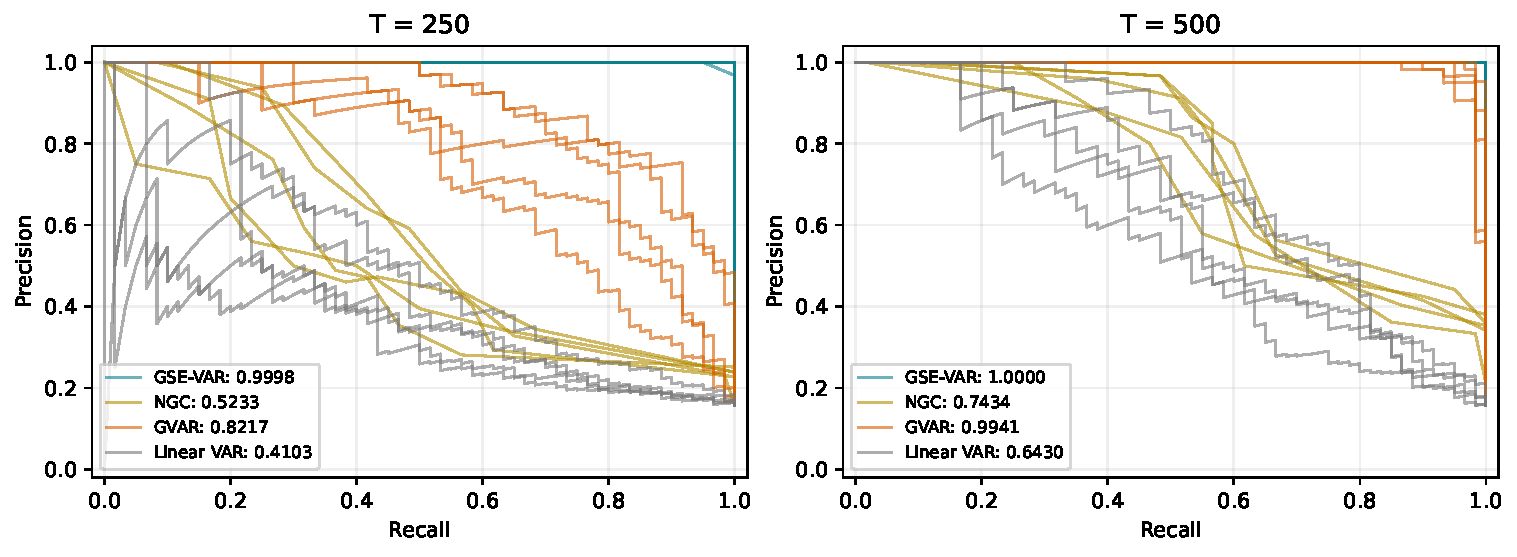
\includegraphics[width=\linewidth]{figures/lorenz_lambda_paths.pdf}
\caption{Lorenz96のPR曲線。各条件の5系列を重ねた。GSE-VARとNGCは正則化10候補で選択された辺、GVARと線形VARはそれぞれ係数強度と負の\(p\)値に対する閾値を変えて求める。線は観測点間を結び、凡例は平均AUPRCを示す。}
\label{fig:lorenz-paths}
\end{figure}

図\ref{fig:lorenz-structures}で選択頻度を示す。GVARの\(T=500\)ではAUPRCが高くても採用グラフには見落としが残り、順位評価と固定グラフの回復は一致しない。

\begin{figure}[!htbp]
\centering
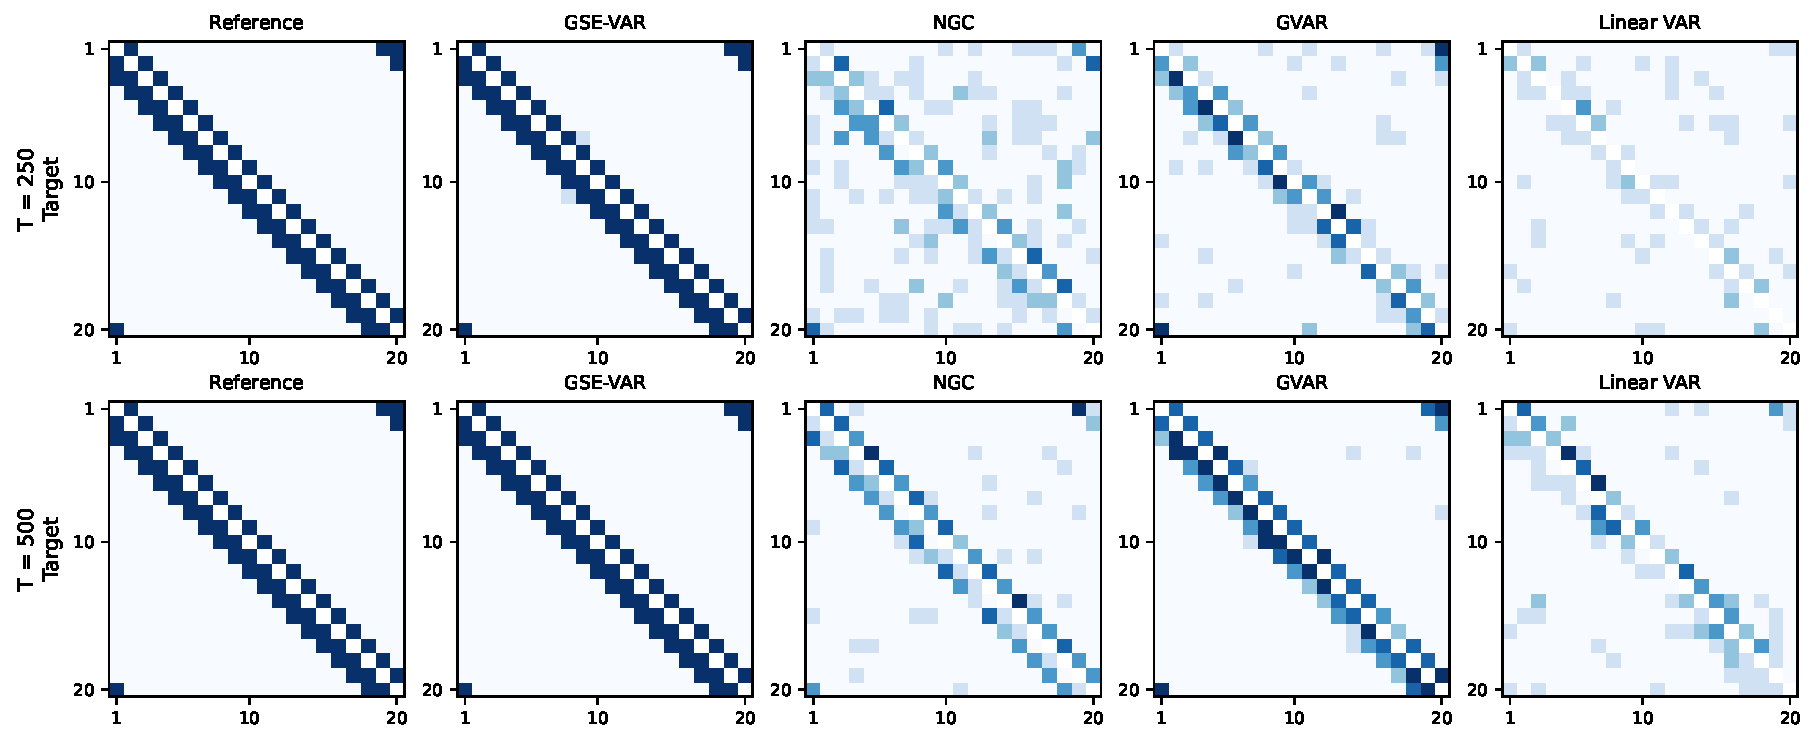
\includegraphics[width=\linewidth]{figures/lorenz_structures.pdf}
\caption{Lorenz96の参照構造と各手法の辺選択頻度。行は予測対象、列は入力系列であり、色は5回の実験で辺が選択された割合を示す。上段は\(T=250\)、下段は\(T=500\)。自己辺は灰色とした。}
\label{fig:lorenz-structures}
\end{figure}

\subsection{線形VAR過程における符号回復}
表\ref{tab:linear-results}では、両系列長とも線形VARの平均符号BAが最も高い。GSE-VARは\(T=250,500\)でそれぞれ\(0.900\)、\(0.975\)となり、GVARを上回った。

\begin{table}[H]
\centering\small
\caption{線形VARの符号回復。10系列の平均\(\pm\)標本標準偏差。正・負のBAはそれぞれの符号を陽性として算出し、その平均を主指標とする。各条件・指標の最大平均値を太字とした。}
\label{tab:linear-results}
\setlength{\tabcolsep}{4pt}
\begin{tabular}{rlrrr}
\toprule
\(T\)&手法&\(\mathrm{BA}_{pos}\)&\(\mathrm{BA}_{neg}\)&平均符号BA\\
\midrule
250&GSE-VAR&\(0.908\pm0.169\)&\(0.892\pm0.167\)&\(0.900\pm0.129\)\\
&GVAR&\(0.883\pm0.172\)&\(0.877\pm0.178\)&\(0.880\pm0.157\)\\
&線形VAR&\(\mathbf{0.995}\pm0.014\)&\(\mathbf{0.990}\pm0.021\)&\(\mathbf{0.993}\pm0.012\)\\
\midrule
500&GSE-VAR&\(0.975\pm0.079\)&\(0.975\pm0.079\)&\(0.975\pm0.053\)\\
&GVAR&\(0.895\pm0.172\)&\(0.912\pm0.178\)&\(0.903\pm0.140\)\\
&線形VAR&\(\mathbf{0.995}\pm0.014\)&\(\mathbf{0.990}\pm0.020\)&\(\mathbf{0.993}\pm0.011\)\\
\bottomrule
\end{tabular}
\end{table}

図\ref{fig:linear-coefficients}に全12非自己係数を示す。GSE-VARでは符号が一致しても係数が大きく変動する場合がある。

\begin{figure}[H]
\centering
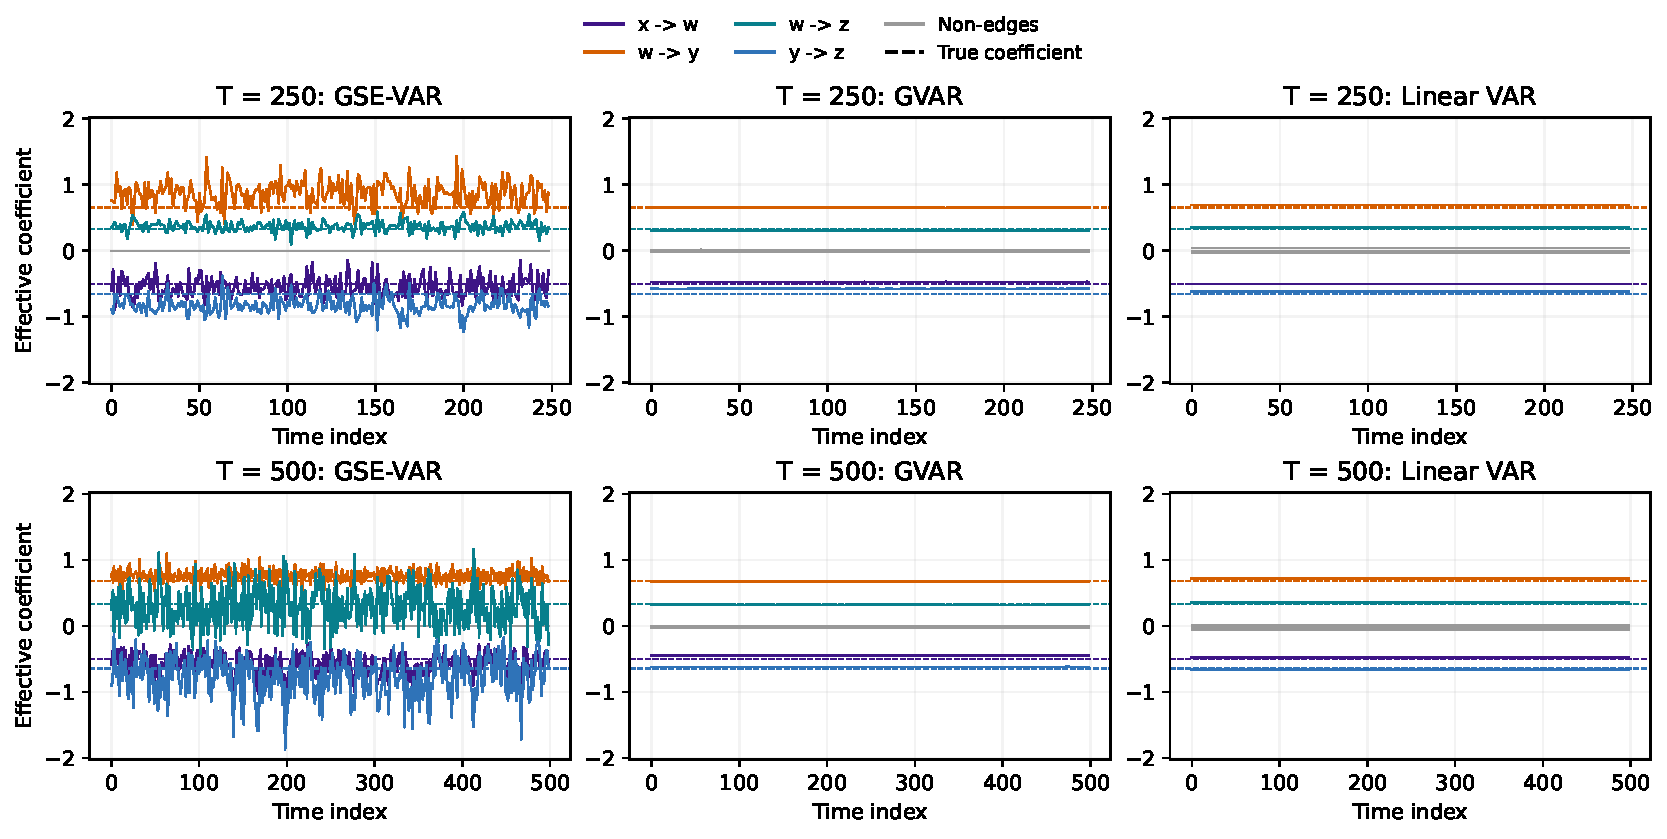
\includegraphics[width=.94\linewidth]{figures/linear_coefficients.pdf}
\caption{線形VARの全12非自己係数。上段は\(T=250\)、下段は\(T=500\)の第1系列。左からGSE-VAR、GVAR、線形VAR。色付き実線は4真辺、灰色実線は8非辺、破線は標準化後の真値を示す。全6パネルの縦軸を共通とし、平滑化や値の切り捨ては行っていない。}
\label{fig:linear-coefficients}
\end{figure}

\section{限界}
\label{sec:limitations}
命題\ref{prop:noncausality}はモデル内の入力非依存性を保証する一方、真の構造の回復は変数集合、ラグ数、表現力、標本数に依存し、相関する入力が予測を代替すれば選択辺も変わり得る。Lorenz96で確認したのは、独立した予備系列の正解構造で設定を選んだ条件での性能である。未知構造で同等の回復を実現できるとは限らず、予測損失の小ささだけでは選択グラフの正しさを確認できない。

Favoritaでは単一店舗の12カテゴリと一つの学習初期値に対象が限られる。販促、価格、祝日、在庫、来店者数などを明示的に条件付けていないため、選択辺が共通要因を反映する可能性がある。曜日調整後も残る季節性や非定常性も推定に影響する。初期値や店舗を変えた再現性、外部情報を加えた構造の安定性は、本稿の結果からは判断できない。

有効係数とヤコビアンの対応は観測状態上で調べられ、介入効果の同定には追加の因果仮定を要する。対象・ラグ別の生成器が表す交互作用の範囲は同一ラグ内に限られる。

\section{結論}
入力依存係数と入力経路の厳密な除去を両立するGSE-VARを定式化し、共通の二値ゲートによる推定モデル上の非因果性の十分条件を示した。Bernoulliゲートの選択確率に期待L0正則化を課し、DisARMによる不偏勾配推定とAdamで学習する。Lorenz96では系列長500の全5系列で参照構造を回復し、線形VARでは同じ系列長の平均符号BAが\(0.975\)となった。Favoritaでは予測依存を7本の経路として記述できた。外生入力を別枝で扱うVARXにも同じ学習方法を適用できる。

\clearpage
\appendix
% !TeX root = ../main.tex
\section{Favorita販売データへの適用}
\label{sec:application}
\subsection{分析目的とデータ}
エクアドルの小売企業Corporación Favoritaの販売データ\citep{favoritadata}を用いる。訓練中に全12カテゴリの正販売日の割合が\(80\%\)以上で、各系列に変動がある店舗のうち最小番号の店舗1（Quito）を選んだ。対象カテゴリは図\ref{fig:favorita-mse}に示す。

2016年7月1日から2017年2月28日を訓練、2017年3月1日から4月30日を検証、5月1日から8月15日をテストとする。欠測の2016年12月25日は補間せず、7日ラグの窓全体が観測される場合のみ用いる。訓練は欠測前後で区切り、検証61時点、テスト107時点を評価する。

販売量を\(y_{j,t}\)、曜日を\(d(t)\)として、入力を
\begin{equation}
 x_{j,t}=\frac{\log(1+y_{j,t})-m_{j,d(t)}}{s_j}
 \label{eq:favorita-transform}
\end{equation}
へ変換する。\(m_{j,d}\)は訓練区間における曜日別の対数販売量の平均、\(s_j\)は曜日平均を除いた訓練残差の標準偏差である。訓練で求めた変換を検証・テストに固定し、外生変数は入力しない。

\subsection{候補設定と検証による選択}
GSE-VAR、NGCのcMLP\citep{tank2022}、線形VAR(SGL)を比較し、最大ラグを7日とする。GSE-VARは隠れ層1層・幅8、平滑化係数\(0.01\)、重み減衰\(0.001\)、初期選択確率\(0.5\)とする。尺度\(s\in\{0,0.3,1,2,3,4,6,10,20,40\}\)を\(\lambda_0=s/(7\times12^2)\)に換算し、係数・ゲート学習率の組\((0.003,0.03),(0.001,0.01),(0.001,0.03)\)と合わせて30候補を比較する。cMLPは隠れ層1層・幅100、L2係数\(0.01\)とし、階層グループ正則化係数\(\{0,0.001,0.003,0.01,0.03,0.1,0.3,0.5,1,10\}\)と学習率\(\{0.01,0.003\}\)の20候補を近接勾配法で学習する。両ニューラルモデルは最大5000エポック、初期200エポックまでは20、その後は100エポックごとに検証する。線形VARはL1係数\(10^{-4}\)、グループ係数\(\{0,10^{-5},3\times10^{-5},10^{-4},3\times10^{-4},10^{-3},0.003,0.01,0.03,0.1\}\)の10候補とする。検証MSE最小の候補・チェックポイントを採用し、同点ではエポック数、候補番号の順で選ぶ。

採用されたGSE-VARは\(s=2\)、学習率の組\((0.003,0.03)\)、1400エポック、cMLPは正則化係数\(0.1\)、学習率\(0.01\)、5000エポックであり、線形VARのグループ係数は\(0.01\)であった。検証最良モデルを再推定せずテストで評価する。学習初期値は42とする。

\subsection{予測誤差と選択構造}
目的変数\(j\)のテストMSEと、全変数をまとめたMSEを
\begin{equation}
 \mathrm{MSE}_j=\frac{1}{N_{\mathrm{test}}}\sum_t(\widehat x_{j,t}-x_{j,t})^2,
 \qquad
 \mathrm{MSE}=\frac{1}{12}\sum_{j=1}^{12}\mathrm{MSE}_j
 \label{eq:favorita-mse}
\end{equation}
と定める。全体のRMSEは\(\sqrt{\mathrm{MSE}}\)である。表\ref{tab:favorita-overall}のとおり、GSE-VAR、cMLP、線形VARのテストMSEはそれぞれ\(0.4620,0.4727,0.4703\)、ラグを統合した非自己辺数は7本、39本、66本であった。GSE-VARは三手法の中で最も低いテストMSEと少ない選択辺数を示した。

\begin{table}[!htbp]
\centering\small
\caption{Favoritaのモデル選択とテスト評価。誤差は標準化尺度、辺数は自己辺を除く。各手法1モデルの値である。}
\label{tab:favorita-overall}
\begin{tabular}{lrrrr}
\toprule
手法&検証MSE&テストMSE&テストRMSE&非自己辺数\\
\midrule
GSE-VAR&0.4533&0.4620&0.6797&7\\
cMLP&0.4617&0.4727&0.6875&39\\
線形VAR(SGL)&0.4810&0.4703&0.6858&66\\
\bottomrule
\end{tabular}
\end{table}



図\ref{fig:favorita-mse}では調理済食品と魚介の誤差が大きい。GSE-VARは酒類で線形VARより低いMSEを示す一方、冷凍食品では線形VARが低い。

\begin{figure}[!htbp]
\centering
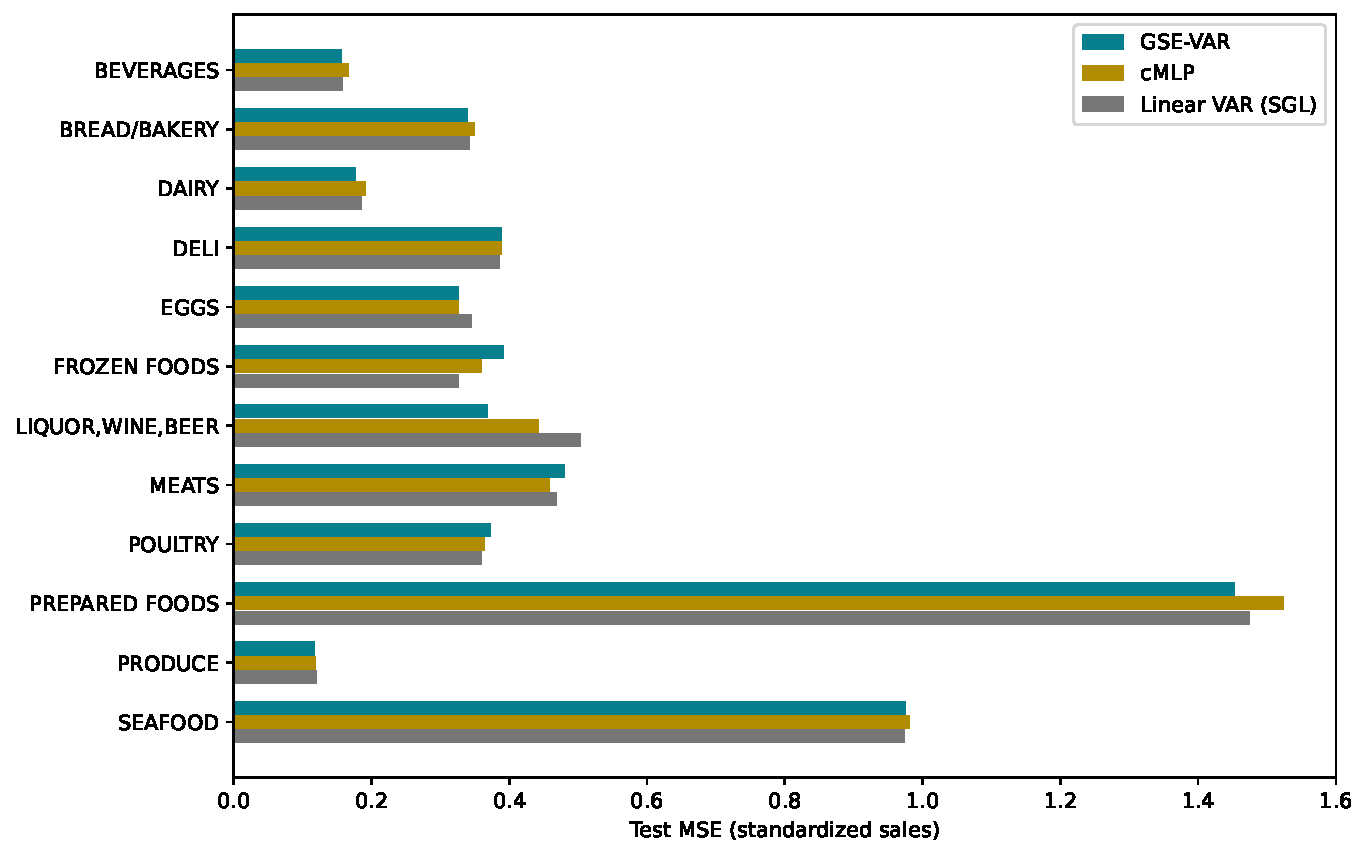
\includegraphics[width=.94\linewidth]{figures/favorita_target_mse.pdf}
\caption{目的変数別テストMSE。三手法で同一の107時点を評価し、曜日調整した対数販売量の標準化尺度で比較する。}
\label{fig:favorita-mse}
\end{figure}

\subsection{カテゴリ間の関係の記述}
図\ref{fig:favorita-structures}に三手法の選択構造、図\ref{fig:favorita-links}にGSE-VARの7本の非自己選択経路を示す。GSE-VARの各辺はいずれも一つのラグで構成され、モデル内で利用可能な予測経路を表す。

\begin{figure}[H]
\centering
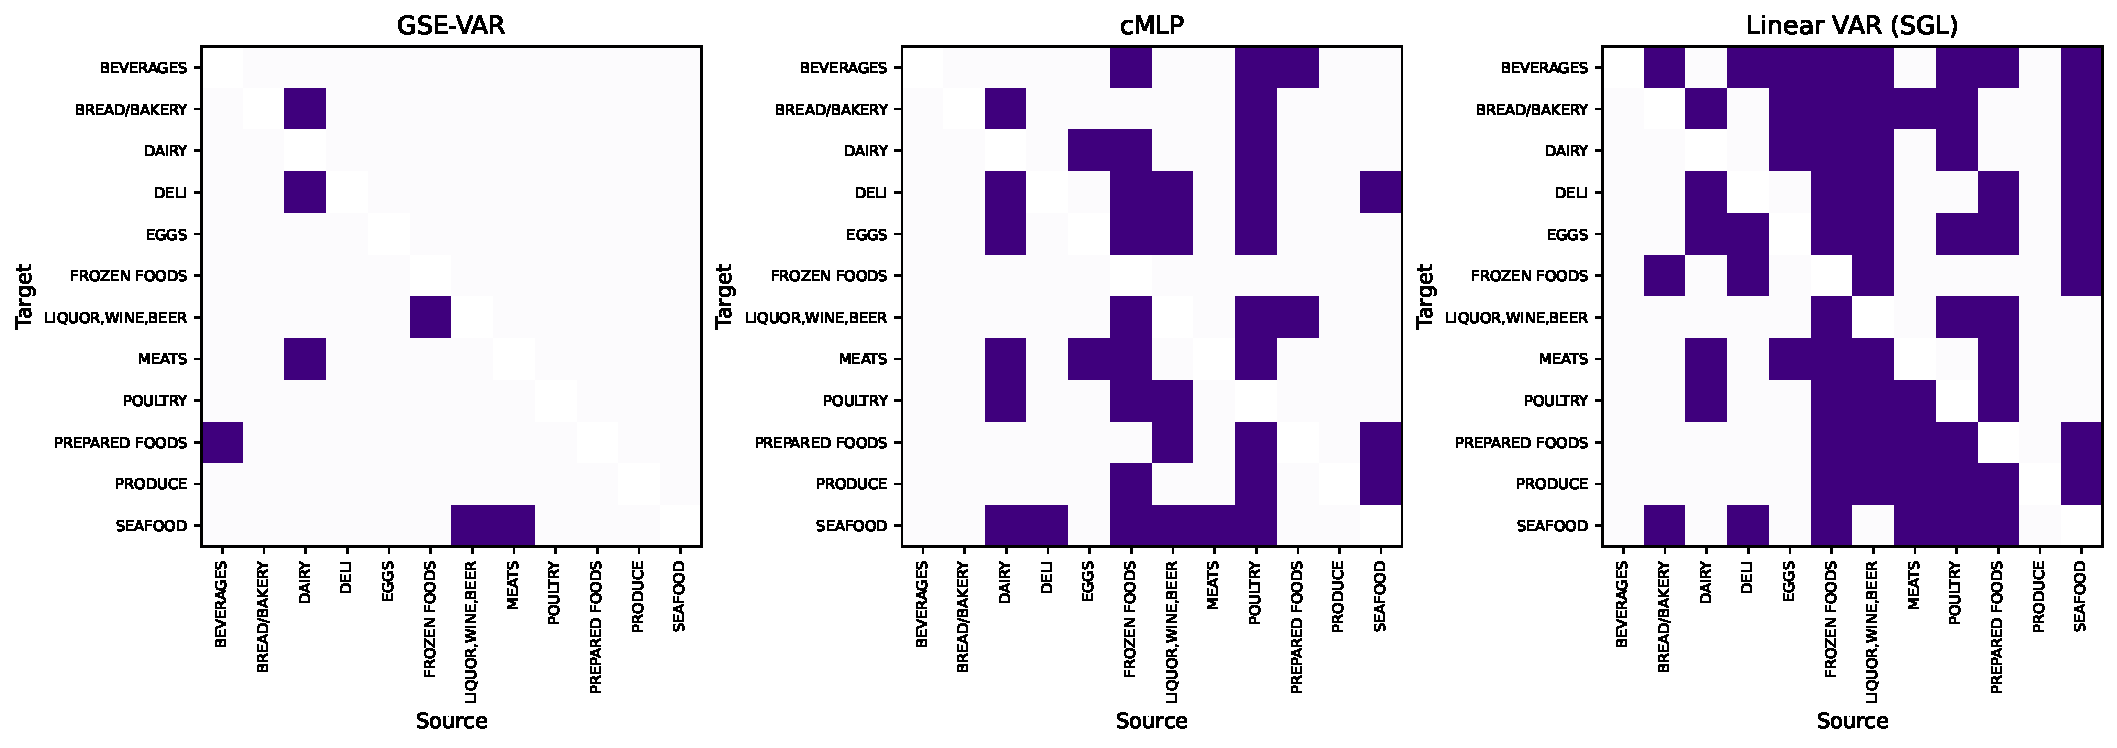
\includegraphics[width=\linewidth]{figures/favorita_structures.pdf}
\caption{Favoritaのラグ統合選択構造。左からGSE-VAR、cMLP、線形VAR。行が予測対象、列が入力で、紫色は少なくとも一つのラグが選択された変数対を示す。cMLPは入力層の非零重み、線形VARは非零係数から辺を抽出し、自己辺は表示から除いた。}
\label{fig:favorita-structures}
\end{figure}

係数の符号はテスト時点の\(80\%\)以上で正なら正、\(80\%\)以上で負なら負、他は混在とする。酒類から魚介は混在、残る6経路は正であった。

\begin{figure}[H]
\centering
\resizebox{\linewidth}{!}{\begin{tikzpicture}[box/.style={draw=violet!80!black,fill=violet!5,rounded corners=2pt,minimum width=3.1cm,minimum height=.65cm,font=\small},route/.style={-{Stealth[length=2.5mm]},line width=.9pt,draw=violet!80!black},every edge quotes/.style={font=\footnotesize}]
\node[box] (dairy) at (-4,2.2) {乳製品};
\node[box] (bread) at (0.3,3.2) {パン・ベーカリー};
\node[box] (deli) at (0.3,1.9) {デリ食品};
\node[box] (meat) at (0.3,0.6) {肉類};
\node[box] (seafood) at (5,0.6) {魚介};
\node[box] (frozen) at (-4,-1) {冷凍食品};
\node[box] (liquor) at (0.3,-1) {酒類};
\node[box] (beverages) at (-4,-2.5) {飲料};
\node[box] (prepared) at (5,-2.5) {調理済食品};
\draw[route] (beverages.east) -- node[above,font=\footnotesize,fill=white,inner sep=1pt,text=violet!80!black] {\(+0.361\)（7日前）} (prepared.west);
\draw[route] (dairy.east) -- node[above,font=\footnotesize,fill=white,inner sep=1pt,text=violet!80!black] {\(+0.306\)} (bread.west);
\draw[route] (dairy.east) -- node[below,font=\footnotesize,fill=white,inner sep=1pt,text=violet!80!black] {\(+0.437\)} (deli.west);
\draw[route] (frozen.east) -- node[above,font=\footnotesize,fill=white,inner sep=1pt,text=violet!80!black] {\(+0.146\)} (liquor.west);
\draw[route] (dairy.south east) -- node[below,sloped,font=\footnotesize,fill=white,inner sep=1pt,text=violet!80!black] {\(+0.369\)} (meat.north west);
\draw[route,dashed,draw=gray] (liquor.east) -- node[below,sloped,font=\footnotesize,fill=white,inner sep=1pt,text=gray] {\(+0.035\)} (seafood.south west);
\draw[route] (meat.east) -- node[above,font=\footnotesize,fill=white,inner sep=1pt,text=violet!80!black] {\(+0.233\)} (seafood.west);
\end{tikzpicture}
}
\caption{GSE-VARの非自己選択経路。矢印は入力から予測対象への向きを示す。数値は標準化尺度の107テスト時点における係数の中央値。飲料から調理済食品は7日前、他は1日前の入力であり、破線は符号が混在する経路を表す。}
\label{fig:favorita-links}
\end{figure}

係数は予測式上の重みを表す。図\ref{fig:favorita-links}のように、カテゴリ名・ラグ・係数を組み合わせることで、予測を担う経路を具体的に検討できる。局所感度との対応には式\eqref{eq:jacobian}を用い、共通する購買動向や販促の影響は第\ref{sec:limitations}節の課題として扱う。

\phantomsection
\addcontentsline{toc}{section}{参考文献}
\begingroup
\interlinepenalty=10000
\bibliographystyle{abbrvnat}
\bibliography{references}
\endgroup
\end{document}
